\chapter{Конструкторская часть}

В данном разделе будут представлены схемы последовательной и параллельной работы стадий конвейера

\section{Требования к программному обеспечению}

К программе предъявлены ряд требований:

\begin{itemize}[label=---]
	\item наличие меню для выбора запускаемого режима работы конвейера --- последовательного или параллельного — или выхода из программ;
	\item предоставление интерфейса для ввода линейного размера обрабатываемых матриц и числа заявок;
	\item работа с массивами и <<нативными>> потоками;
	\item формирование файла с логом работы конвейера, логирование событий обработки должно происходить после окончания работы, собственно, конвейера.
\end{itemize}

\section{Разработка алгоритмов}

На рисунке~\ref{fig:linear} представлен последовательный алгоритм работы стадий конвейера.

\begin{figure}[h]
	\centering
	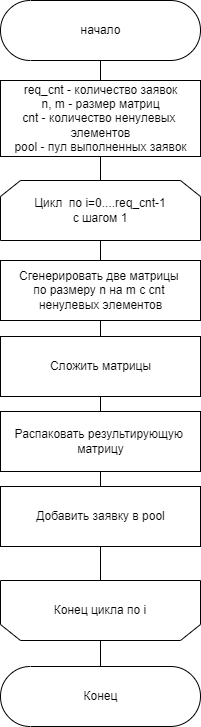
\includegraphics[height=0.85\textheight]{img/linear.png}
	\caption{Схема алгоритма последовательной конвейерной обработки}
	\label{fig:linear}
\end{figure}

\clearpage

Параллельная работа будет реализована с помощью добавления 3-х вспомогательных потоков, где каждый поток отвечает за свою стадию обработки.
Вспомогательному потоку в числе аргументов в качестве структуры будут переданы:
\begin{itemize}
	\item две матрицы в РСФ;
	\item результирующая матрица сложения двух матриц в РСФ;
	\item матрица в классическом представлении для распаковки;
	\item временные отметки начала и конца выполнения стадии обработки заявки.
\end{itemize}

На рисунке~\ref{fig:thr} представлена схема главного потока при параллельной работе стадий конвейера.

\begin{figure}[h]
	\centering
	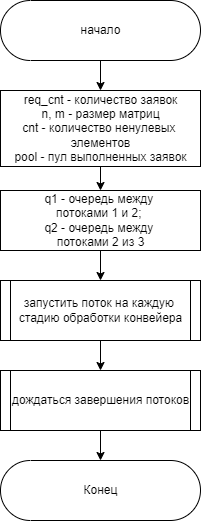
\includegraphics[height=0.5\textheight]{img/thr.png}
	\caption{Схема параллельной конвейерной обработки}
	\label{fig:thr}
\end{figure}

На рисунках \ref{fig:gen}--\ref{fig:unpack} представлены схемы алгоритмов каждого из обработчиков (потоков) при параллельной работе.

\begin{figure}[h]
	\centering
	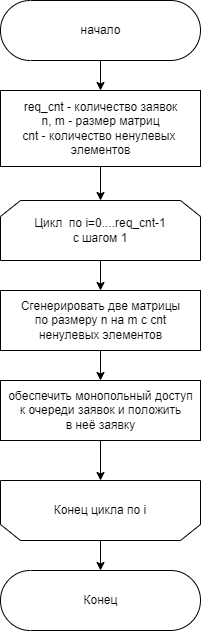
\includegraphics[height=0.85\textheight]{img/gen.png}
	\caption{Схема алгоритма потока 1}
	\label{fig:gen}
\end{figure}

\begin{figure}[h]
	\centering
	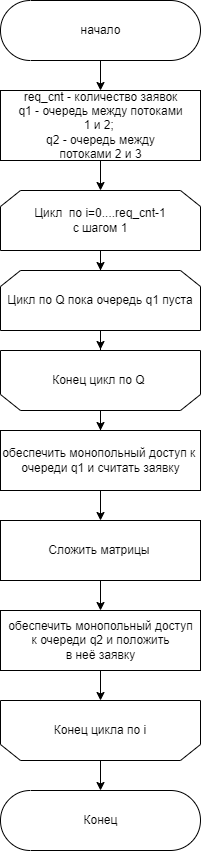
\includegraphics[height=0.85\textheight]{img/sum.png}
	\caption{Схема алгоритма потока 2}
	\label{fig:sum}
\end{figure}

\begin{figure}[h]
	\centering
	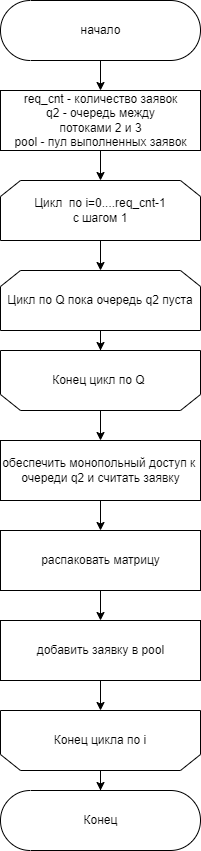
\includegraphics[height=0.85\textheight]{img/unpack.png}
	\caption{Схема алгоритма потока 3}
	\label{fig:unpack}
\end{figure}

\clearpage

\section*{Вывод}
В данном разделе были представлены схемы последовательной и параллельной работы стадий конвейера.